% Keep the supplied class unchanged. pdfLaTeX uses its original spot colours.
% Tectonic/XeTeX preview uses the identical declared CMYK colour because the
% template's 2006 spotcolor package only implements pdfTeX primitives.
\RequirePackage{iftex}
\ifXeTeX
  \RequirePackage[T1]{fontenc}
  \RequirePackage{color}
  \makeatletter
  \@namedef{ver@spotcolor.sty}{2026/09/16 XeTeX preview compatibility}
  \newcommand\NewSpotColorSpace[1]{}
  \newcommand\AddSpotColor[4]{}
  \newcommand\SetPageColorSpace[1]{}
  \def\color@spotcolor#1#2{\color@cmyk#1{1,0.3,0,0.2}}
  \makeatother
\fi

\documentclass[nolineno]{ieeeaccess}
\usepackage{cite}
\usepackage{amsmath,amssymb,amsfonts}
\usepackage{graphicx,booktabs,tabularx,array}
\usepackage{textcomp,xurl}
\usepackage[hidelinks]{hyperref}
\usepackage{iftex,etoolbox,needspace,placeins}
\makeatletter
\InputIfFileExists{t1pcr.fd}{}{}
\DeclareFontShape{T1}{pcr}{n}{n}{<->ssub*pcr/m/n}{}
\DeclareFontShape{T1}{formata}{m}{sl}{<->ssub*formata/m/it}{}
\makeatother
\patchcmd{\IEEEbiographynophoto}{\vskip 4\baselineskip plus 1fil minus 0\baselineskip}{\vskip 2\baselineskip}{}{}
\makeatletter
\newcommand{\submissionfooter}{\hbox to\textwidth{\hfill\footerpagefont\thepage}}
\apptocmd{\ps@titlepage}{\let\@oddfoot\submissionfooter\let\@evenfoot\submissionfooter}{}{}
\apptocmd{\ps@headings}{\let\@oddfoot\submissionfooter\let\@evenfoot\submissionfooter}{}{}
\patchcmd{\@maketitle}{Digital Object Identifier\space\@doi}{}{}{\PackageError{paper}{DOI suppression failed}{Check template title macro}}
\makeatother
\ifXeTeX
\special{pdf:mapfile t1-times.map}
\special{pdf:mapfile t1-formata.map}
\special{pdf:mapfile t1-giovannistd.map}
\fi
\graphicspath{{figures/}}
\newlength{\paperabstractwidth}
\setlength{\paperabstractwidth}{\dimexpr\titlewidth-10pt\relax}
\let\abstractwidth\paperabstractwidth
\setcounter{dbltopnumber}{3}
\renewcommand{\dbltopfraction}{.9}
\renewcommand{\topfraction}{.9}
\renewcommand{\textfraction}{.08}
\newcolumntype{L}{>{\raggedright\arraybackslash}X}
\newcommand{\rankE}{r_{\mathrm{E}}}
\newcommand{\AIdraftingnote}{\footnote{Drafting and code assistance: OpenAI Codex \cite{codex}; see the Acknowledgment for scope.}}
% Generated by build_assets.py; values are retained advantage, not accuracy.
\newcommand{\aggregationrows}{%
Original tokens & 100.00 & 100.00 & 100.00 & 100.00 \\
One global mean & 61.14 & 62.12 & 61.23 & 62.62 \\
Eight band means & 70.42 & 72.62 & 54.20 & 58.24 \\
Four column means & 76.39 & 72.47 & 75.90 & 64.95 \\
Five spatial moments & 76.05 & 81.89 & 68.39 & 81.55 \\
Five random modes & 65.47 & 66.43 & 61.07 & 62.87 \\
Train-position template & 7.75 & 6.31 & -29.19 & -27.77 \\
Template + mean residual & 75.09 & 74.69 & 52.85 & 52.84 \\
Template + five residual moments & 81.76 & 82.17 & 65.82 & 65.29 \\
}

\hypersetup{pdftitle={Local Texture Evidence and Aggregation in Compact Tyre Inspection: A Reproducible Limited-Data Study},pdfauthor={Sreenivasa Reddy Edara, Shanmukesh Bonala},pdfsubject={Author-review research manuscript; not a physical wear or safety validation}}
\begin{document}
\raggedbottom
\pagestyle{headings}
\history{}
\doi{}
\title{Local Texture Evidence and Aggregation in Compact Tyre Inspection: A Reproducible Limited-Data Study}
\author{\uppercase{Sreenivasa Reddy Edara}\authorrefmark{1}, AND
\uppercase{Shanmukesh Bonala}\authorrefmark{2}}
\address[1]{School of Computer Science and Engineering, VIT-AP University, Amaravati, India (e-mail: sreenivasareddy.e@vitap.ac.in)}
\address[2]{School of Computer Science and Engineering, VIT-AP University, Amaravati, India (e-mail: shanmukesh.23BCE20070@vitapstudent.ac.in)}
\corresp{Corresponding author: Sreenivasa Reddy Edara (e-mail: sreenivasareddy.e@vitap.ac.in).}
\begin{abstract}
Compact vision systems for tyre inspection can achieve high mask agreement while failing to transfer mileage-proxy predictions across tyres. Whether their intermediate texture evidence remains useful after spatial aggregation is less clear. This study examines that question using 570 existing images from 12 user-confirmed tyres and a sequence of fully recorded custom-model experiments. A geometry-anchored texture model, TRACE, learns six fixed local image descriptors with 71,022 trainable parameters. At its unselected final endpoint, local reconstruction reduces validation loss by 36.44\% relative to a train-position control, and masked reconstruction improves by 21.63\% over the strongest declared control. Nevertheless, every epoch fails the original global-diversity selection requirements. We therefore conduct a saved-feature study of nine predefined aggregation interventions using unchanged decoder weights, identical target support, and training-only templates. A global mean retains 61.14\% of the original local validation advantage, compared with 81.76\% for a position template plus five residual spatial moments. Retention varies by descriptor and tyre component; orientation errors are especially sensitive. A covariance decomposition shows that only 4.15\% of within-component token variance occupies the constant spatial mode. Invertible scaling and an exploratory mask-layout analysis further show why spectral diversity alone is insufficient evidence of useful texture. The contribution is an auditable analysis of local evidence and aggregation in a limited-data system, rather than a validated physical-wear estimator or a promoted checkpoint.
\end{abstract}
\begin{keywords}
Feature aggregation, image reconstruction, representation analysis, reproducibility, tyre inspection.
\end{keywords}
\titlepgskip=-21pt
\maketitle
\section{Introduction}\label{sec:introduction}
\PARstart{V}{isual} tyre inspection combines several different questions. A system may locate a tyre, identify its tread region, estimate image-relative boundaries, classify a usage-related category, and expose the evidence behind its output. These functions have different supervision and different meanings. A good mask is evidence of region agreement, whereas a reliable physical-wear estimate requires suitable measurements and independent evaluation. Optical tread-depth systems such as TireEye explicitly connect image structure to a physical reference \cite{tireeye}. A classifier trained on mileage categories does not acquire that connection merely by producing a plausible heat map.\AIdraftingnote

The present work grew from a compact, custom multitask system developed for an existing tyre-inspection application. Its dense outputs were useful internally, but mileage-proxy classification transferred poorly to the allocated held-out tyres. Subsequent changes addressed gradient interference, appearance sensitivity, reference exposure, spatial layout, and separation of geometry from texture learning. These revisions supplied informative failures rather than a consistently improving classifier. They also made it possible to ask a narrower question: \emph{does useful local texture evidence survive the operation that converts spatial tokens into a global representation?}

This question matters because reconstruction and representation diagnostics can disagree for structural reasons. A local reconstruction head can read individual tokens without ever using a pooled image vector. Simultaneously, an auxiliary global head can be dominated by one direction of variation. Observing both properties does not constitute a contradiction. Nor does increasing a rank statistic automatically establish better evidence: coordinate scaling changes spectral balance, and a recorded mask layout can contribute variation unrelated to the desired texture content.

We study these issues in TRACE (Texture Reconstruction with Anchored Canonical Evidence), a small model built around frozen predicted geometry and fixed local image descriptors. Its six targets describe contrast, edge energy, orientation, curvature, and contrast occupancy. They are observable image properties, not annotated groove depth or damage. The model improves local and masked reconstruction against the declared controls but never satisfies its original representation-selection requirements. We preserve that outcome and examine the saved final tokens using the same frozen decoder, rather than retraining until a favorable endpoint appears.

The contributions are threefold. First, we document a compact geometry-anchored model and the experimental context that motivated a shift from proxy classification to local texture analysis, including unsuccessful revisions and unchanged selection rules. Second, we formulate a controlled saved-feature assay that compares nine spatial aggregation interventions on identical supported targets, with training-only templates and explicit frozen-head replay accounting. Third, we connect the measured reconstruction losses to descriptor-specific effects, component-centered covariance, invertible scaling, and an exploratory mask-layout association. These analyses distinguish local predictive utility from broad global diversity and identify a constrained future design question.

The study uses 570 images from 12 user-confirmed physical tyres. It is a retrospective, limited-data investigation with only two conservative components in each held-out role. The historical test role was inspected repeatedly during development. Accordingly, its results are descriptive corroboration on a known allocation, not an unbiased estimate from a new external test. We report no new physical-wear accuracy, no independent safety decision, and no newly selected TRACE checkpoint.

\section{Related Work}\label{sec:related}
\subsection{Tyre Inspection and the Meaning of a Target}
Tyre inspection spans physical measurement, region detection, surface defects, and product-level decisions. Petrovi\'{c} et al. studied tread-depth inspection using oriented-gradient features and a support-vector classifier \cite{tread2021}. TireEye uses an optical arrangement and a geometric reference to estimate tread wear \cite{tireeye}. Mignot et al. aggregate defect detections with attention-guided multiple instance learning for manufacturing-quality decisions \cite{mil2025}. These settings motivate local texture and aggregation, but their labels, sensing arrangements, and decision criteria differ from the mileage-proxy labels used here. Their performance values are therefore not directly comparable with this study.\AIdraftingnote

Our earlier project stages provided task-specific classification, segmentation, and boundary models. Standard residual networks \cite{resnet} and transformer-based segmentation \cite{segformer} offer relevant architectural context, but this paper does not present a new benchmark against all such families. The measured Phase 3 sequence instead records how particular application failures motivated subsequent custom components. Its scientific emphasis is the relation between a representation and the information a fixed readout can recover from it.

\subsection{Shared Learning and Inspectable Evidence}
Multitask learning shares parameters across related objectives \cite{caruana}. That sharing can also create optimization conflicts. Gradient surgery addresses interfering task gradients \cite{pcgrad}; we use a separately declared symmetric two-task projection as a paired diagnostic, rather than asserting a new general optimizer. Its unsuccessful outcome motivates explicit separation of geometry and texture parameters in later experiments.

Evidence visualization requires an additional distinction. A map can account exactly for a model's score without identifying a physical cause. Saliency sanity checks demonstrate why visual plausibility alone is insufficient to establish explanation validity \cite{sanity}. Shortcut learning likewise warns that predictive cues can depend on incidental regularities rather than the intended phenomenon \cite{shortcuts}. In this work, additive class maps are described as score accounting, and TRACE descriptors as fixed image evidence. Neither is presented as a validated causal explanation of tyre wear.

\subsection{Masked Prediction and Representation Diversity}
Masked autoencoders learn by reconstructing missing visual content \cite{mae}. MaskFeat further shows the value of predicting fixed descriptors and of local contrast normalization \cite{maskfeat}. TRACE adopts the narrower idea of masked prediction of fixed local fields, using a small convolutional encoder on a tyre-specific atlas. It is not a replication of large-scale MaskFeat training, and it does not inherit those models' transfer results.

Variance--invariance--covariance regularization (VICReg) explicitly combines paired-view invariance, variance control, and covariance regularization \cite{vicreg}; Barlow Twins addresses redundancy through cross-correlation \cite{barlow}. TRACE uses a small auxiliary objective inspired by the former principle. RankMe relates a representation's effective rank to downstream model assessment \cite{rankme}. Our retained implementation instead computes an entropy rank from covariance-energy weights, which square singular values. We define that statistic explicitly and do not equate its numerical values with RankMe. Centered kernel alignment (CKA) supplies a separate way to compare representational similarity \cite{cka}; here it is used only in an exploratory mask-layout analysis.

The gap addressed by this study is operational rather than a new universal representation theorem. We ask how much of a trained local readout's advantage survives prescribed spatial compression, then check whether spectral diagnostics describe the same phenomenon. This combination exposes useful local information that global metrics alone obscure, while retaining the original failed selection outcome.

\Needspace{8\baselineskip}
\section{Data and Evaluation Protocol}\label{sec:data}
\subsection{Existing Data and Conservative Independence}
The fixed collection contains 418 original photographs and 152 extracted frames from videos of three existing mid-category tyres, yielding 570 unique images. The additional frames increase view coverage, not the number of physical subjects. The user identifies 12 distinct physical tyres. This identity record is not an independent forensic audit.\AIdraftingnote

The training allocation contains 386 images, validation 81, and the historical test allocation 103 (Table~\ref{tab:data}). Images carry low-, mid-, or high-mileage proxy categories derived from source odometer folders. Low combines new tyres with the 100--5,000 group; mid contains the 40,000, 70,000, and 90,000 groups; high is the 100,000-plus group. These source labels are not measurements of abrasion. The known tyre allocation is eight/two/two. Unresolved relationships among three mid-category video parents are conservatively merged for component-based analysis. Consequently, the training role has six conservative connected components: one low, one mid, and four high. Their image counts are 67, 249, 60, 5, 3, and 2. This grouping does not assert that the three user-identified mid tyres are physically identical; it prevents uncertain provenance from being treated as independent evidence.

\begin{table}[t]
\caption{Fixed image allocation and supervision. Components are conservative provenance groups, not additional tyres.}\label{tab:data}
\centering\small
\setlength{\tabcolsep}{4pt}
\begin{tabularx}{\columnwidth}{Lrrr}\toprule
Quantity & Train & Validation & Historical test\\\midrule
Images & 386 & 81 & 103\\
Low / mid / high & 67 / 249 / 70 & 40 / 0 / 41 & 62 / 0 / 41\\
User-confirmed tyres & 8 & 2 & 2\\
Conservative components & 6 & 2 & 2\\
Human point images & 70 & 25 & 25\\
Weak point images & 152 & 0 & 0\\
No point target & 164 & 56 & 78\\\bottomrule
\end{tabularx}
\end{table}

Neither held-out role contains mid-category ground truth. Observed-class balanced accuracy (BA) is therefore the mean of low and high recalls, even though a classifier can predict all three categories. It is not three-class coverage. Class and component identity are strongly confounded: each held-out class corresponds to one conservative component per role. Group-aware evaluation is essential in dependent data \cite{groups}; here the small number of independent groups also limits what can be inferred after grouping.

\subsection{Geometry and Annotation Provenance}
The 418 original images have indexed masks, and the 152 frames have polygon-derived masks. Tyre and tread targets are overlapping binary channels. Pixels contradicted by the annotation contract are ignored rather than forced into mutually exclusive classes. A 120-image subset provides six human boundary points per image, allocated 70/25/25. The 152 video frames additionally supply weak polygon-derived point targets, weighted 0.25 during training. These weak targets are not counted as independent human evaluation truth.

Mean Dice describes agreement with available segmentation annotations; horizontal point mean absolute error (MAE) is normalized by image width and evaluated on human point images. Image-relative boundary positions do not provide physical camber, toe, or groove-depth measurements. TRACE uses frozen predicted support, not ground-truth masks at inference. Annotation ignore regions affect target-loss eligibility and do not enter the texture network as observation channels.

\subsection{Development History and Reporting Units}
The Phase 3 ledger contains seven fit families and ten measured fit executions: three TREAD-ONE seeds, two matched paired-diagnostic fits, and one fit each for ATLAS, ATLAS-LC, ATLAS-CONTEXT, GEO, and TRACE. Each execution has 60 epochs and 2,940 optimizer updates, totaling 600 epochs and 29,400 updates. Recovery of an interrupted fit is continuation of that execution. Notebook wrappers, preparation gates, review notebooks, and engineering fixtures are not additional measured models.

Later candidates have one seed each. Their sequence is hypothesis-driven development rather than a factorial or fully seed-replicated comparison. Hyperparameters and selection contracts were frozen separately for each execution, but the overall sequence responded to previously inspected outcomes. Model-selection bias can arise even with a fixed finite validation allocation \cite{selectionbias}. We therefore distinguish validation-selected checkpoints from fixed final endpoints and explicitly acknowledge repeated historical-test inspection. No test-best checkpoint replaces the declared validation choice.

The primary new investigation is post-hoc analysis of retained TRACE evidence. Its nine interventions and arithmetic were recorded before that calculation; they were not prospectively preregistered before the model was trained. The mask-layout addendum was formulated later, after a high masked-token rank was observed, and is labeled exploratory. No image-independent confidence intervals or significance tests are reported: treating the many related images as independent replicates would misrepresent the support. Image means, component summaries, complete counts, and exact losses are reported instead.

\section{Model Sequence and Geometry-Anchored Texture Learning}\label{sec:models}
\subsection{TREAD-ONE and Motivating Diagnostics}
TREAD-ONE is a custom 1,372,159-parameter network trained from scratch at an input resolution of $512\times384$ (height by width). A texture encoder, two context transformer blocks, and shared decoding features support two sigmoid masks, mask-derived boxes, six ordered boundary coordinates, and proxy classification. Twelve nonnegative latent maps are combined with a detached, normalized predicted-tread gate and signed linear class weights. Their additive contributions plus bias reconstruct the class logits. This identity makes score accounting inspectable; it does not establish semantic concepts or input-level causal faithfulness.\AIdraftingnote

The three selected seeds achieved strong internal mask agreement but inconsistent proxy transfer. We therefore evaluated a matched seed-1 shared-gradient intervention. Classification is one task and the weighted dense objective the second. When shared gradients have a negative dot product, each is projected away from the other using the original pair of vectors; the projected gradients are then combined. This is a declared symmetric two-task variant motivated by gradient surgery \cite{pcgrad}. It preserves task routing, but global gradient clipping can still affect the total update. Its results do not support promotion over the matched baseline.

ATLAS then freezes the dense anchor and uses local query/reference evidence for proxy classification. The first version showed appearance sensitivity and repeated exposure to a restricted query set. ATLAS-LC introduces paired local-contrast grayscale inputs, full-source-hash self-exclusion from an 18-image reference bank, and square-root component sampling. ATLAS-CONTEXT adds a zero-initialized, bounded positional residual over a frozen LC prior. These changes address distinct observed weaknesses, yet none recovers low-category recall on the historical test role. They are context for the texture question, not interchangeable causal ablations of one factor.

GEO, the geometry-first revision, separates geometry, texture, and annotation-error parameters. Its bounded geometry adjustment preserves mask quality and modestly improves internal point error. Its texture representation remains ineligible under the joint gate. A 64-dimensional diversity projector is also difficult to interpret with centered batches of eight, whose covariance rank cannot exceed seven. This dimensional constraint is a feasibility observation, not proof that it caused the failed representation. TRACE retains GEO's fixed final geometry and reduces the auxiliary projector to six dimensions while replacing learned texture targets with explicit fixed descriptors.

\subsection{Canonical Atlas and Fixed Targets}\label{sec:targets}
TRACE uses 1,399,227 frozen geometry parameters and 71,022 trainable texture parameters, for 1,470,249 total. The geometry consists of the selected TREAD-ONE anchor and GEO's final geometry adjustment. GEO's final state was not selected under its original joint gate; its use here is an explicitly frozen research dependency, not a retrospective promotion.

Predicted tyre--tread support defines a canonical $512\times256$ atlas, sampled with bilinear red--green--blue (RGB) values and nearest-neighbor support. Source rows narrower than 16 pixels are unavailable. The atlas contains an $8\times4$ grid of nonoverlapping $64\times64$ tiles. All dimensions in this paper use height before width.

Within each tile, grayscale $g=(R+G+B)/3$ is locally standardized using masked $9\times9$ means and standard deviations, with denominator floor 0.02. The result is clipped to $[-3,3]$, divided by three, and multiplied by observation support to obtain $z$. Tile-local Sobel derivatives $d_x,d_y$, divided by eight, supply edge information. Table~\ref{tab:targets} defines the six fields. These fixed descriptors encode canonical image structure; their thresholds and coordinates have no calibrated physical-wear interpretation.

\begin{table}[t]
\caption{Six fixed image fields before cell averaging. $e=d_x^2+d_y^2$; $\Delta$ is the four-neighbor Laplacian.}\label{tab:targets}
\centering\small
\begin{tabularx}{\columnwidth}{lL}\toprule
Field & Definition\\\midrule
Contrast & $z$\\
Gradient energy & $\sqrt{e}$\\
Orientation axis & $(d_x^2-d_y^2)/(e+0.0025)$\\
Orientation cross & $2d_xd_y/(e+0.0025)$\\
Relative curvature & $\min\{1,|\Delta z/4|/(|d_x|+|d_y|+0.05)\}$\\
Contrast occupancy & $\mathbf{1}[|z|>0.15]$\\\bottomrule
\end{tabularx}
\end{table}

Loss support intersects predicted support with the complement of the annotation ignore mask. An $11\times11$ erosion with invalid padding removes pixels whose radius-five contrast/derivative dependency is not valid. Each tile is reduced to $4\times4$ cells of $16\times16$ pixels. A cell is available only when at least 64 valid pixels remain; the count weights its loss. Missing targets have zero weight and are not treated as observed zeros.

Channel means and population standard deviations are fitted on the 386 training images using 64-bit floating-point (FP64) accumulation and stored in 32-bit floating point (FP32), with a standard-deviation floor of 0.001. Targets are standardized with these statistics. A separate train-position mean is retained for each tile/cell/channel, including its count and availability. Neither statistic uses validation or historical-test targets.

\subsection{Local, Contextual, and Global Paths}\label{sec:architecture}
Figure~\ref{fig:architecture} separates the paths that are easily conflated in aggregate metrics. Input channels are $z,d_x,d_y$, and gradient magnitude. Four stride-two convolution blocks, with channel widths 16, 24, 32, and 48, Group Normalization, and sigmoid linear unit (SiLU) activations, produce a 48-dimensional vector per tile after spatial averaging. Let $Z\in\mathbb{R}^{32\times48}$ denote these local tokens. A shared multilayer decoder
\begin{equation}
 D:\mathbb{R}^{48}\rightarrow\mathbb{R}^{96}\rightarrow\mathbb{R}^{96}
\end{equation}
uses SiLU between its two linear layers and reshapes each output to six $4\times4$ fields. The local prediction is $D(Z)$, before cross-tile mixing or global pooling.

\begin{figure*}[t]
\centering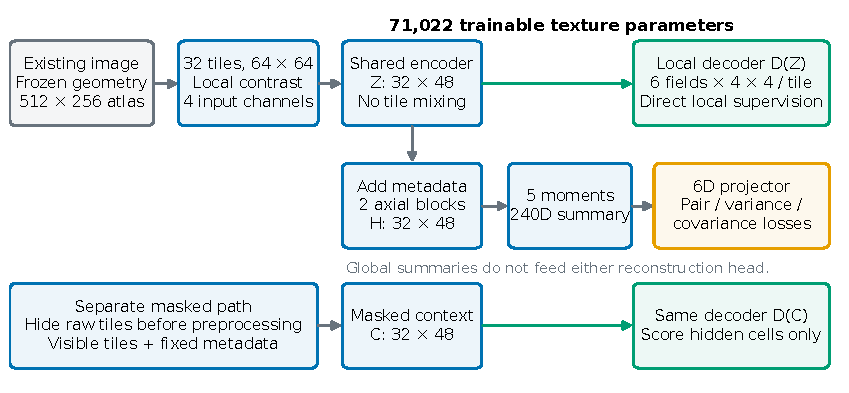
\includegraphics[width=\textwidth]{architecture.pdf}
\caption{Actual TRACE information flow. The local reconstruction head reads unpooled tokens $Z$. The masked head reads contextual tokens $C$ from a separately masked observation path. The full-context tokens $H$ feed an auxiliary global summary. Thus local reconstruction can be useful while the global summary fails diversity requirements. Geometry remains frozen in all paths.}\label{fig:architecture}
\end{figure*}

Row, column, and predicted coverage metadata are projected into 48 dimensions. Two residual axial blocks mix depthwise row and column convolutions with pointwise channel transformations, producing full-context tokens $H$. Coverage is normalized within each supported band and then equally across supported bands to yield nonnegative masses $m_t$ with $\sum_t m_t=1$. The recorded local mean is $\sum_t m_t Z_t$; the full-context mean is $\sum_t m_t H_t$.

The actual global descriptor contains five moments of $H$. Coordinates $y$ and $x$ are the fixed linearly spaced values from $-1$ to $1$ on the eight rows and four columns. With
\begin{equation}
 b_t=[1,y_t,x_t,y_tx_t,y_t^2-1/3],
\end{equation}
the descriptor concatenates $\sum_t m_t b_{tk}H_t$ for $k=1,\ldots,5$, yielding 240 dimensions. The constant $1/3$ is source-defined; the discrete basis is not assumed orthogonal under each image's masses. A $240\rightarrow48\rightarrow6$ projector supplies the paired-view diversity objective. It does not feed the local decoder.

\subsection{Masking, Objective, and Original Selection}\label{sec:training}
Two deterministic image/view-addressed photometric views vary brightness, contrast, and gamma in $[0.9,1.1]$, while targets remain those of the clean atlas. A separate plan hides one supported tile in a band when at least two exist, for at most eight hidden tiles. Hidden raw RGB and observation support are removed \emph{before} preprocessing and encoding. A learned mask token and the permitted position/coverage metadata then enter the context blocks, producing $C$. The masked prediction $D(C)$ is scored on hidden supported cells. Clean targets, annotation ignore masks, and full-path encodings are not context inputs. However, the fixed predicted geometry was computed from the full image; the masking boundary is conditional on that geometry and is not a claim of image-level causal occlusion.

The loss is
\begin{equation}\label{eq:loss}
\begin{split}
\mathcal{L}={}&\mathcal{L}_{\mathrm{local}}+\mathcal{L}_{\mathrm{mask}}
 +0.1\mathcal{L}_{\mathrm{pair}}\\
 &+0.1\mathcal{L}_{\mathrm{var}}+0.01\mathcal{L}_{\mathrm{cov}}.
\end{split}
\end{equation}
Reconstruction uses Smooth L1 with transition $\beta=0.1$ on standardized fields. Valid-pixel counts weight cells; channels are averaged within each image and available images are then averaged equally. The two views' terms are averaged. The pair term is mean squared error between six-dimensional projected vectors. With unbiased sample covariance $S$ ($n-1$ denominator), the variance term averages $\max(0,0.1-\sqrt{S_{jj}+10^{-4}})$, and the covariance term is $\sum_{j\ne k}S_{jk}^2/(6\cdot5)$. Diversity losses require at least seven eligible rows, making six-dimensional centered variation feasible in batches of eight. This is an adaptation inspired by VICReg, not a claim to reproduce its original recipe.

TRACE uses AdamW with learning rate 0.001, weight decay 0.0001, gradient clipping at one, FP32 arithmetic, and no scheduler or gradient scaler. One seed is run for 60 epochs and 49 updates per epoch. Each epoch has 386 primary image draws and six deterministic padding draws, yielding 23,520 draws in total. Kaggle provides two T4 graphics processing units (GPUs): geometry-cache construction uses the second device and texture optimization the first. This is not distributed data-parallel training.

Three controls predict hidden descriptors: the training channel mean, the training position mean, and the mean of visible descriptors in the same band. All are scored on the same intersection of supported hidden cells and control availability. The original validation contract requires at least 90\% primary exposure and 95\% common control coverage; at least 5\% masked improvement over \emph{each} control; at least 10\% local improvement over the position control; projector rank at least four and median standard deviation at least 0.05; local-mean and spatial-summary ranks at least four; and within-component local/spatial ranks at least two. Finite-state and frozen-geometry provenance checks also apply. Eligible checkpoints minimize masked loss divided by the strongest control loss, plus 0.1 times paired cosine distance, retaining the earliest tie. No epoch is eligible, so the selected endpoint remains unavailable. The final epoch is studied as a fixed diagnostic endpoint.

\section{Saved-Feature Aggregation Study}\label{sec:aggregation}
\subsection{Endpoint, Inputs, and Replay Boundary}
We analyze the fixed final TRACE endpoint at epoch 60, update 2,940. The retained evidence contains $Z$, $H$, and $C$ for 570 images and two recorded views, each of shape $32\times48$, together with masses, mask plans, fixed targets, target weights, and frozen decoder/projector parameters. No new photo, photometric view, geometry forward pass, image-encoder forward pass, or optimizer update is introduced. The primary intervention sweep performs 656,640 frozen decoder-token readouts. Bridge verification adds 72,960 decoder-token and 1,140 projector-vector readouts. Calling it saved-feature analysis therefore does not mean zero computation.\AIdraftingnote

View 0 is the primary clean observation. View 1 is a retained sensitivity view; its appearance factors and mask plan both differ, so a change between views cannot be attributed to appearance alone. Training-only templates and scales use view 0. The validation and historical-test roles contain all 32 supported tiles per image. Two training images have missing tiles, with at least 28 supported. Fixed-grid training spectra can consequently include placeholder effects; our principal covariance interpretation uses the complete-support held-out roles.

\subsection{Nine Fixed Interventions}
For one image/view and one token layer, let $X\in\mathbb{R}^{32\times48}$, $M=\operatorname{diag}(m)$, and $B\in\mathbb{R}^{32\times k}$ be a prescribed spatial basis. The mass-weighted projection is
\begin{equation}\label{eq:projection}
 \mathcal{P}_B(X)=B(B^{\mathsf T}MB)^+B^{\mathsf T}MX,
\end{equation}
where the Moore--Penrose pseudoinverse uses relative cutoff $10^{-10}$. This reconstructs a token at every original position from the permitted spatial modes. It changes neither feature channels nor decoder parameters.

The nine interventions are: (1) original tokens; (2) one constant mode, equivalent to a global mass-weighted mean; (3) eight row-band indicators; (4) four column indicators; (5) the five source-defined spatial moments; (6) a constant plus four fixed random zero-sum orthogonal modes; (7) a train-position feature template; (8) that template plus a constant-mode residual; and (9) that template plus five residual moments. Random modes are generated once with seed 462225 using Gaussian draws, mean removal, and QR factorization. They are a dimension-matched spatial control, not an optimized random search.

Let $T$ be the unweighted per-position feature mean over supported training images, fitted separately for each layer. The final two variants are
\begin{equation}
 \widehat X=T+\mathcal{P}_B(X-T).
\end{equation}
The template is a feature statistic, not a target-fitted neural model. All held-out fitting is excluded. Bands, columns, moments, and random modes have different dimensions or structure; the analysis asks what each prescribed compression retains, not whether one has superior capacity after matched retraining.

The unchanged decoder $D$ reads each transformed $Z$ for local reconstruction and each transformed $C$ for masked reconstruction. The same supported cells, hidden cells, and train-position-control availability are used for every variant. Full-context $H$ participates in representation diagnostics and in verification of the actual global branch; it is not substituted into the local reconstruction headline.

\subsection{Loss and Retained Advantage}\label{sec:utility}
For predictions $p_{icuv}$ and standardized targets $t_{icuv}$, define Smooth L1
\begin{equation}
 h_\beta(a)=\begin{cases}a^2/(2\beta),&|a|<\beta,\\ |a|-\beta/2,&\text{otherwise},\end{cases}
\end{equation}
with $\beta=0.1$. Cell weights are valid-pixel counts on the common support. The image loss averages channels after weighted cell reduction; role-level loss averages available images equally. Thus a large tyre region does not automatically dominate a small one.

Let $L_0$ be the loss of original tokens, $L_v$ the loss under intervention $v$, and $L_{\mathrm{pos}}$ the fixed train-position target control on the same support. We report
\begin{equation}\label{eq:retention}
 R_v=\frac{L_{\mathrm{pos}}-L_v}{L_{\mathrm{pos}}-L_0}.
\end{equation}
For a positive original advantage, $R_v=1$ retains that advantage, $R_v=0$ matches the position control, and a negative value is worse than that control. It is not a classification accuracy, a proportion of physically meaningful information, or a universal information measure. Small original margins can make channel-specific $R_v$ unstable; we therefore show absolute channel losses as well.

The 21.63\% original masked-improvement headline uses the \emph{strongest declared control}, the visible-band mean, whereas~\eqref{eq:retention} consistently uses the train-position control. These denominators answer different questions and are not interchanged. The transformed tokens may also lie outside the decoder's training distribution. Their loss measures compatibility and recoverable evidence under the \emph{fixed} readout, not all information that a newly trained decoder could exploit.

\subsection{Spectral and Component Diagnostics}\label{sec:spectra}
For a role-centered image-feature matrix with covariance eigenvalues $\lambda_j\geq0$, define
\begin{equation}\label{eq:rank}
 p_j=\frac{\lambda_j}{\sum_\ell\lambda_\ell},\qquad
 \rankE=\exp\!\left(-\sum_jp_j\log p_j\right).
\end{equation}
For the saved-feature diagnostics, numerical eigenvalues below $10^{-14}$ of total energy are excluded. Original selection retains its native positive-eigenvalue treatment; no gate is recomputed with a changed rule. This is covariance-energy entropy rank. Since $\lambda_j$ is proportional to squared singular value, it differs from singular-value-weighted effective rank. Leading-energy fraction, coordinate standard deviations, and dimensions accompany it. Concatenated 1,536-dimensional tokens and pooled 48-dimensional means have different rank ceilings; their comparison is a mechanism diagnostic, not matched model performance.

We also center each conservative component separately. The between-component fraction is $1-V_{\mathrm{within}}/V_{\mathrm{total}}$, using the same covariance trace convention. This identifies where variance lies, without making component identity a permissible deployment input. In these data, class and component are confounded, so removing identity indiscriminately could also remove category-associated variation.

For a spatial decomposition, fix a single mass vector $r$ to the mean recorded training mass, normalized to sum to one. Using the same role and centering policy, let
\begin{equation}
 K_{tu}=\frac{1}{N-1}\sum_i\langle\widetilde X_{it},\widetilde X_{iu}\rangle.
\end{equation}
Then the weighted tile variance, constant-mode variance, and spatial residual obey
\begin{equation}
\begin{aligned}
 V_{\mathrm{tile}}&=\sum_t r_tK_{tt},\\
 V_{\mathrm{mean}}&=r^{\mathsf T}Kr.
\end{aligned}
\end{equation}
\begin{align}
 V_{\mathrm{res}}&=\frac{1}{N-1}\sum_{i,t}r_t\left\|\widetilde X_{it}-\sum_u r_u\widetilde X_{iu}\right\|^2,\\[-3pt]
 V_{\mathrm{tile}}&=V_{\mathrm{mean}}+V_{\mathrm{res}}.\label{eq:partition}
\end{align}
Using fixed $r$ makes this identity interpretable. It differs deliberately from the per-image masses used for actual network pooling and reconstruction interventions. Diagonal and cross-position covariance contributions are retained separately.

Finally, we standardize each global feature coordinate using only training-view-0 mean and standard deviation, with floor $10^{-3}$. The inverse transformation is checked. A rank change under this invertible rescaling demonstrates sensitivity to coordinates; it cannot add information to the vector.

\subsection{Exploratory Mask-Layout Association}
After observing high rank in masked tokens, we added a separate diagnostic comparing recorded 32-position hidden indicators with full-context $H$, masked-context $C$, their difference $C-H$, and the actual projector output. For centered Gram matrices $A$ and $B$, linear CKA is
\begin{equation}
 \operatorname{CKA}(A,B)=\frac{\langle A,B\rangle_F}{\|A\|_F\|B\|_F}.
\end{equation}
Component-centered versions remove component means before constructing the Grams. This is an association with a deterministic image-addressed plan, not a randomized masking experiment. CKA is not an explained-variance percentage. The actual projector reads full-context $H$, so a strong association in $C-H$ cannot by itself explain the projector's failed diversity gate.

\section{Results}\label{sec:results}
\subsection{Dense Agreement Does Not Resolve Proxy Transfer}
Table~\ref{tab:trajectory} and Fig.~\ref{fig:classification} summarize the development context. Across the three validation-selected TREAD-ONE seeds, historical-test mean Dice averages 97.978\% and human point MAE 1.189\% of image width. Observed-class BA averages only 34.146\%; the selected seed values are 50.000\%, 2.439\%, and 50.000\%. All three miss every low-category image (0/62). The exported TREAD-ONE checkpoint remains seed 3, epoch 20, chosen by the recorded validation rule. Its availability as an application component is not evidence that its proxy predictions generalize.\AIdraftingnote

\begin{table*}[t]
\caption{Development context on fixed allocations. Selected endpoints follow each original validation rule; final means epoch 60. BA is observed-class balanced accuracy on the 103-image historical test. These serial experiments are not a factorial ablation.}\label{tab:trajectory}
\centering\small
\begin{tabularx}{\textwidth}{LllrrL}\toprule
Experiment & Fits & Endpoint & Val. BA (\%) & Hist. BA (\%) & Main observation\\\midrule
TREAD-ONE r1 & 3 & Selected, seeds 1/2/3 & 55 / 82.5 / 100 & 50 / 2.439 / 50 & Dense agreement does not imply proxy transfer.\\
Paired baseline & 1 & Selected, epoch 23 & 55.00 & 50.000 & Matched seed-1 reference.\\
Shared projection & 1 & Selected, epoch 17 & 83.75 & 17.073 & Dense point error also worsens.\\
ATLAS v1 & 1 & Selected, epoch 18 & 50.00 & 50.000 & Low $\rightarrow$ mid; grayscale/dimming sensitivity.\\
ATLAS-LC & 1 & Selected, epoch 7 & 56.25 & 50.000 & Selected NLL improves; low recall remains zero.\\
ATLAS-CONTEXT & 1 & Selected, epoch 7 & 50.00 & 50.000 & Position sensitivity without better transfer.\\
GEO & 1 & Final; selected unavailable & --- & --- & Geometry floor 60/60; representation eligibility 0/60.\\
TRACE & 1 & Final; selected unavailable & --- & --- & Local/masked utility 60/60; global diversity 0/60.\\\bottomrule
\end{tabularx}
\end{table*}

\begin{figure*}[t]
\centering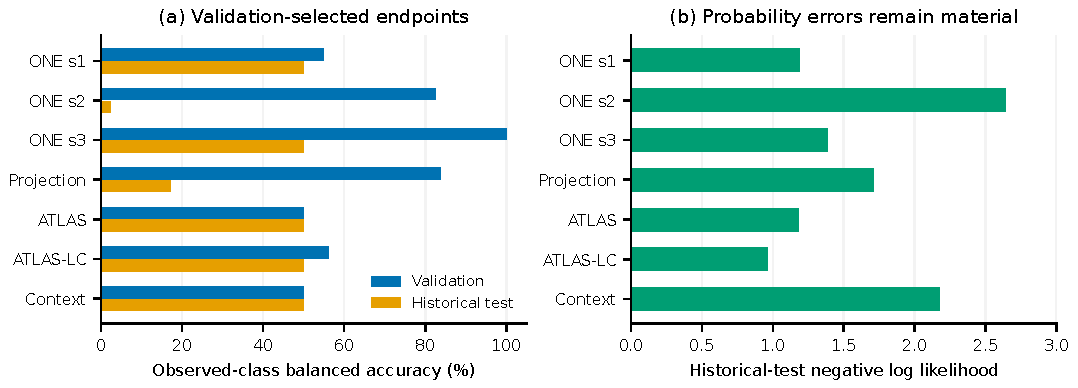
\includegraphics[width=\textwidth]{classification.pdf}
\caption{Validation-selected classifier endpoints on the same historical allocations. ONE s1--s3 are the three TREAD-ONE seeds; Projection is the paired shared-gradient candidate. Later candidates have one seed. NLL is the three-output negative log likelihood on the historical test. Repeated development use prevents an independent-test interpretation.}\label{fig:classification}
\end{figure*}

The shared-gradient candidate intervenes on 91.84\% of its updates but reduces selected BA from 50.000\% to 17.073\%, while human point MAE rises from 1.067\% to 1.885\% of width. This matched result does not support the intervention for this run. It also does not establish that all gradient-conflict methods fail in tyre inspection.

ATLAS, LC, and CONTEXT each retain 50\% historical BA: low recall is 0/62 and high recall 41/41. ATLAS predicts the low group as mid. LC's selected negative log likelihood (NLL) improves from 1.1783 to 0.9613, whereas CONTEXT reaches 2.1748. Probability errors therefore change despite identical endpoint BA, consistent with the need to examine more than hard decisions \cite{calibration}. LC's grayscale stability is partly by construction. CONTEXT responds to layout changes, but that response is not evidence of useful classification. These observations justify the narrower texture investigation without proving a single cause of the proxy failures.

GEO's validation geometry moves from Dice 0.9898659 and point MAE 0.0080854 of width to 0.9898623 and 0.0076622. The 5.23\% relative point reduction is about 0.163 pixels at width 384 and should not be inflated into a physical-accuracy claim. Its final masked reconstruction improves only 4.03\% over the stated mean control, below its 5\% threshold, and its projector rank is 1.0387. No GEO epoch satisfies the joint selection contract.

\subsection{TRACE Learns Local Fields but Remains Unselected}
Table~\ref{tab:trace} gives final TRACE values. Local validation loss is 0.421632 against a train-position loss of 0.663375, a 36.44\% reduction. Masked validation loss is 0.467383 against 0.691031 for the channel mean, 0.662256 for the position mean, and 0.596403 for the visible-band mean. The gain against the strongest aggregate control is 21.63\%. The historical-test counterpart is 17.85\%. Each of the 81 validation images and 103 historical-test images beats all three controls for its final clean-view recorded mask plan; 81/81 and 98/103, respectively, exceed 5\% against every control. These are within-image evidence comparisons, not independent tyre-level success rates.

\begin{table*}[t]
\caption{TRACE final clean-view reconstruction and original validation gate diagnostics. Losses are equal-image standardized Smooth L1.}\label{tab:trace}
\centering\small
\begin{tabularx}{\textwidth}{LrrLrr}\toprule
Reconstruction & Validation & Hist. test & Validation diagnostic & Value & Floor\\\midrule
Local model loss & 0.421632 & 0.412205 & Projector rank & 1.0225 & $\geq4$\\
Local position control & 0.663375 & 0.662712 & Local mean rank & 1.2296 & $\geq4$\\
Local reduction (\%) & 36.44 & 37.80 & Spatial rank & 1.2489 & $\geq4$\\
Masked model loss & 0.467383 & 0.472012 & Projector std. median & 0.0961 & $\geq0.05$\\
Masked visible-band control & 0.596403 & 0.574568 & Within local rank & 9.7824 & $\geq2$\\
Masked reduction (\%) & 21.63 & 17.85 & Within spatial rank & 11.2722 & $\geq2$\\\bottomrule
\end{tabularx}
\end{table*}

Utility, exposure, coverage, finite-state, frozen-geometry, and within-component checks pass at all 60 validation epochs. The projector and encoder/global diversity checks pass at none (Fig.~\ref{fig:training}). The final six-dimensional projector has adequate median amplitude (0.0961) but rank only 1.0225. Likewise, local and spatial pooled ranks remain 1.2296 and 1.2489. Thus amplitude is not the missing property, and the original selected endpoint remains unavailable. We analyze the final state without relaxing these gates.

\begin{figure*}[t]
\centering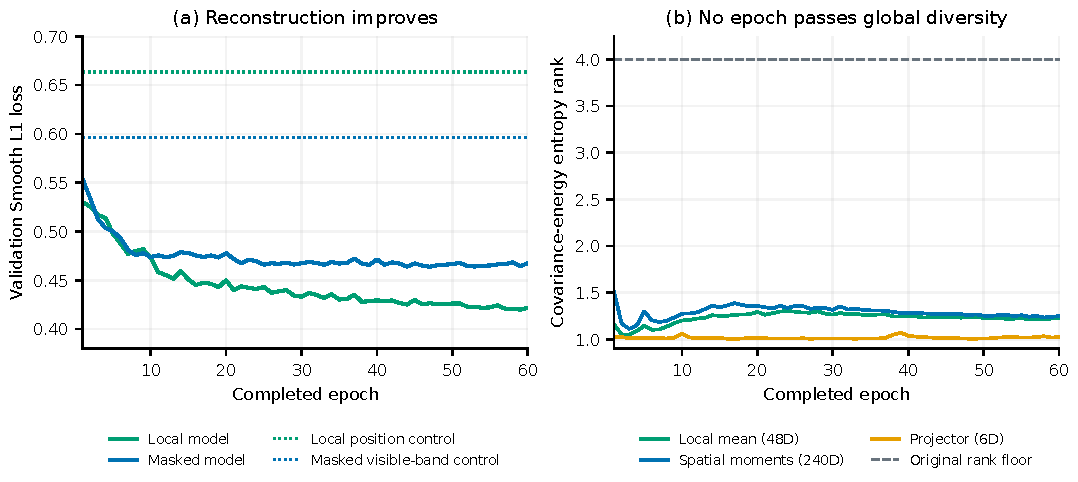
\includegraphics[width=\textwidth]{training.pdf}
\caption{All 60 recorded TRACE validation epochs. Reconstruction improves against fixed controls, while all three global rank traces remain below their original floor. The selected endpoint is unavailable throughout; the final state is used only for the saved-feature diagnosis.}\label{fig:training}
\end{figure*}

\subsection{What Survives Spatial Compression?}
Table~\ref{tab:aggregation} and Fig.~\ref{fig:aggregation} report all nine interventions. A global mean retains 61.14\% of the original local validation advantage and 62.12\% on the historical test. Five fixed moments retain 76.05\% and 81.89\%. A training-position template alone retains only 7.75\% and 6.31\%, whereas the template plus five residual moments retains 81.76\% and 82.17\%. Position-typical features alone therefore do not explain the original local readout's utility, but position plus image-specific residual structure preserves substantially more than a global mean.

\begin{table*}[t]
\caption{Retained advantage $100R_v$ over the train-position target control (\%). Original tokens define 100\%; negative values are worse than the control. All variants use identical target support and the unchanged decoder. These are frozen-head counterfactuals, not trained architecture comparisons.}\label{tab:aggregation}
\centering\small
\begin{tabular}{lrrrr}\toprule
 & \multicolumn{2}{c}{Local branch $Z$} & \multicolumn{2}{c}{Masked branch $C$}\\
Intervention & Validation & Hist. test & Validation & Hist. test\\\midrule
\aggregationrows
\bottomrule\end{tabular}
\end{table*}

\begin{figure*}[t]
\centering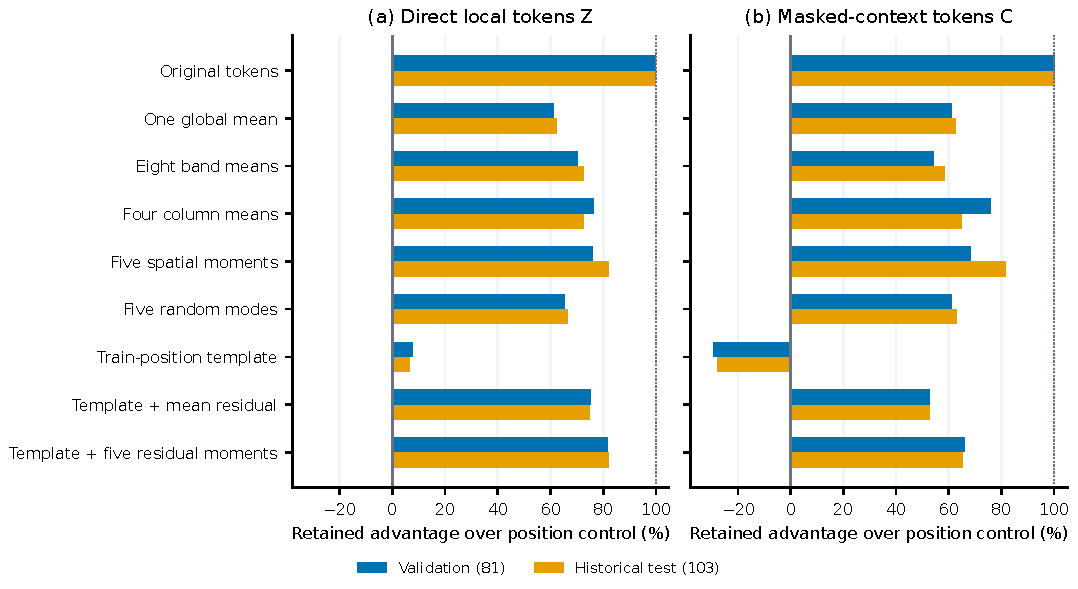
\includegraphics[width=\textwidth]{aggregation.pdf}
\caption{Retained reconstruction advantage under all nine fixed interventions. A global mean loses useful local readout performance. Residual moments preserve more local utility, but they are not uniformly best for the masked task. The training-position template by itself is weak locally and worse than the position-target control on hidden cells.}\label{fig:aggregation}
\end{figure*}

Five random modes retain 65.47\% of local validation advantage, below the five prescribed spatial moments. This one fixed random basis is a control, not a distribution over random projections. Eight band means retain 70.42\%, while four column means retain 76.39\%; the number of modes alone does not order their utility.

The masked branch gives a different ordering. Four column means retain 75.90\% on validation, compared with 68.39\% for five moments, 61.23\% for a global mean, and 65.82\% for template plus residual moments. On the historical test, raw moments retain 81.55\% but the template-residual variant retains 65.29\%. The pure template is below the position-target control in both roles. No single aggregation dominates every task and component, and we do not select an architecture from the most favorable historical-test number.

\subsection{Descriptor and Component Dependence}
Figure~\ref{fig:descriptor} separates six descriptor losses from the aggregate headline. For local validation orientation-axis targets, global averaging raises loss from 0.385328 to 0.585783; residual moments recover it to 0.454548. For orientation-cross targets, the mean's loss is 0.790882, worse than the position control's 0.667389, compared with 0.616969 originally and 0.650077 for residual moments. Contrast also degrades under averaging, from 0.575280 to 0.627355, and is not substantially recovered by residual moments (0.626081). Gradient energy and occupancy are less sensitive in their absolute changes. These differences argue for descriptor-aware evidence retention rather than one global rank target. Figure~\ref{fig:qualitative} illustrates the original and compressed readouts using the lexicographically first validation image in each observed proxy class, without ranking examples by prediction quality.

\begin{figure*}[t]
\centering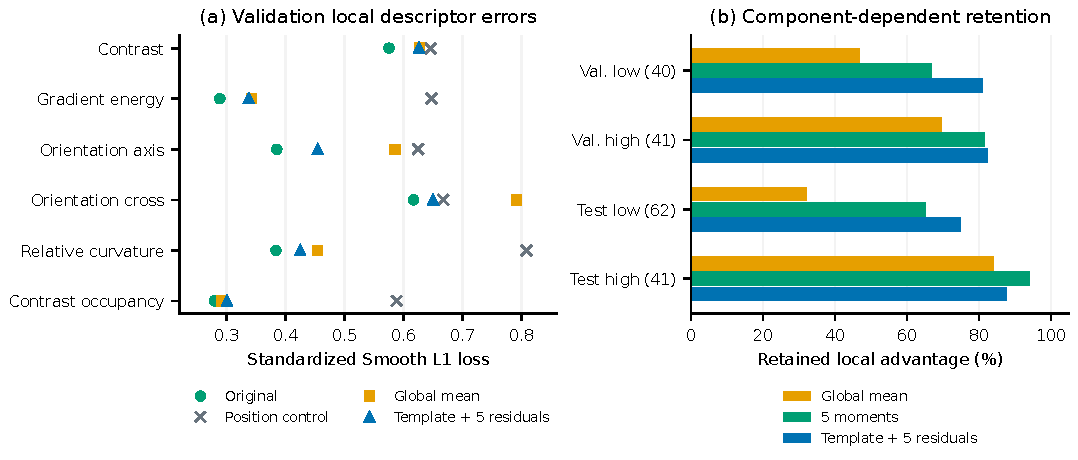
\includegraphics[width=\textwidth]{descriptor_groups.pdf}
\caption{Absolute descriptor loss and component-level local retention for clean view 0. The left panel avoids unstable percentage interpretations when the original control margin is small. The right panel shows that global averaging is more damaging for the historical low component than for the high component. Components coincide with class within each held-out role; this does not isolate a class mechanism.}\label{fig:descriptor}
\end{figure*}

\begin{figure*}[t]
\centering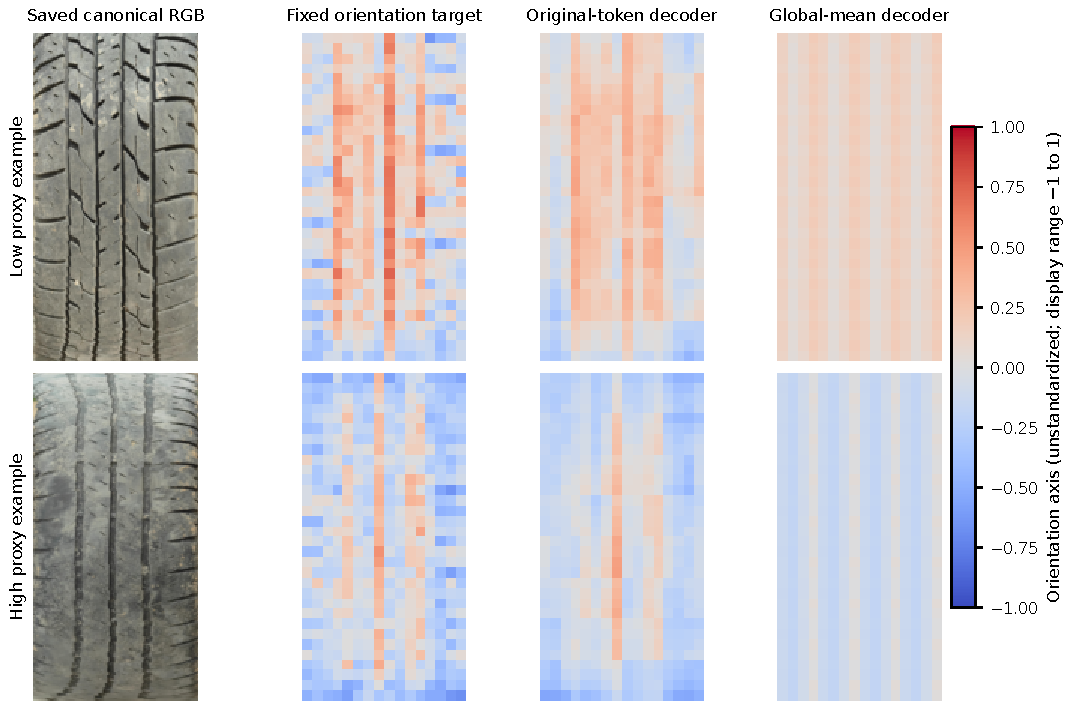
\includegraphics[width=\textwidth]{qualitative.pdf}
\caption{Two deterministic validation examples from the saved canonical atlas and orientation-axis fields. Each row uses the first image identifier in its observed proxy class, not a best/worst error selection. The target and predictions are returned to the raw descriptor scale; colors saturate outside $[-1,1]$ for display only, and unsupported cells are white. Original and global-mean decoder weights are identical. These fields describe image orientation, not groove depth or wear.}\label{fig:qualitative}
\end{figure*}

The historical-test low component retains only 32.03\% of local advantage under a mean, versus 84.02\% for high. Five raw moments retain 65.08\% and 94.13\%, while template plus residual moments retain 74.82\% and 87.52\%. For masked reconstruction the mean retains 23.16\% on low and 81.04\% on high. Such component dependence is consistent with nonuniform loss of local evidence. It does not prove that pooling caused the earlier low-class classification failures: TRACE has a different objective, the interventions are post-hoc, and identity remains confounded with class.

\subsection{Covariance Explains a Distinction, Not Semantic Quality}
Figure~\ref{fig:representation}(a) shows that concatenated local tokens have validation rank 3.4734, falling to 2.4163 after full-context mixing. The local mean has rank 1.2296, actual context moments 1.2489, and actual projector 1.0225. Hence representation concentration is already affected by context; the final averaging operation is not the only transformation implicated by these diagnostics.

After component centering, concatenated local rank is 20.090 and local-mean rank 9.782. Between-component differences account for 96.78\% of local-mean variance, 96.56\% of context-moment variance, and 99.35\% of projector variance. The few coherent component differences dominate global energy even though smaller within-component directions remain. A low total rank should therefore not be interpreted as an exactly constant vector or absence of all local structure.

The fixed training-mass partition in Fig.~\ref{fig:representation}(b) places 30.10\% of total local-token variance in the constant spatial mode, but only 4.15\% after component centering. The corresponding mean off-diagonal position correlations are 0.2731 and 0.0095. Thus most within-component token variation lies outside the constant mode and tends to cancel under averaging. The remaining 95.85\% is a variance fraction, \emph{not} a fraction of useful wear information. Reconstruction measurements, rather than this covariance identity alone, establish the narrower loss of fixed-readout utility.

\begin{figure*}[t]
\centering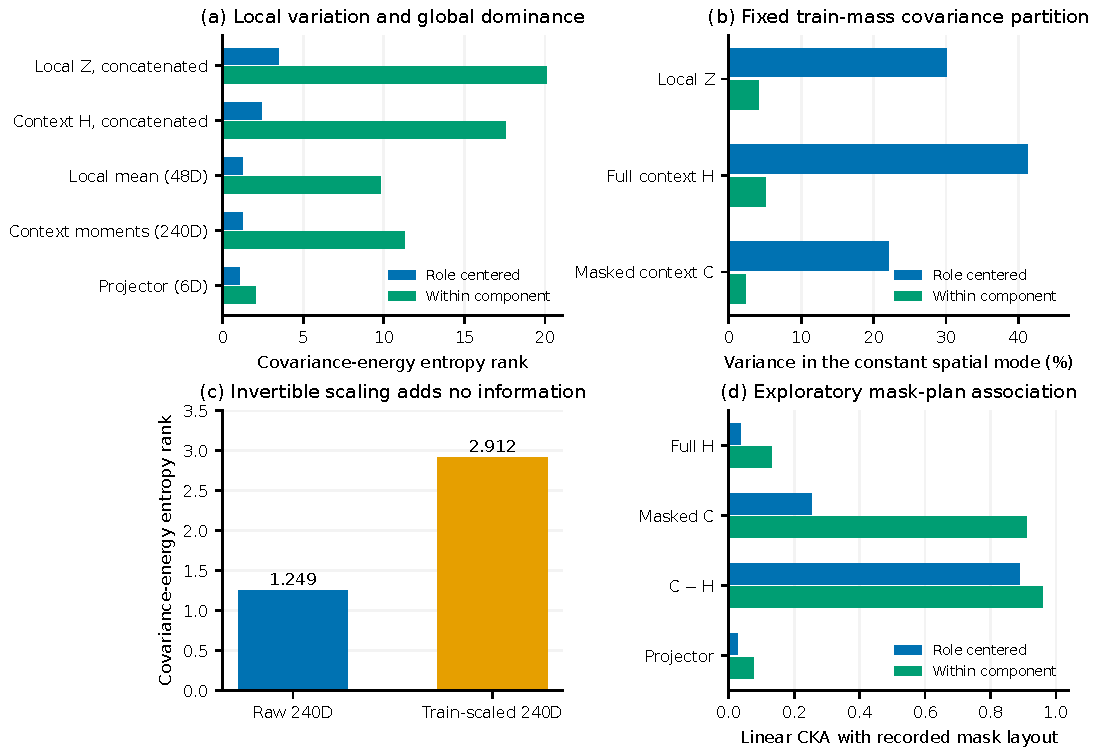
\includegraphics[width=\textwidth]{representation.pdf}
\caption{Validation representation diagnostics for clean view 0. (a) Total and within-component covariance-energy entropy ranks have different interpretations and dimensional ceilings. (b) The fixed train-mass partition isolates the constant spatial mode. (c) Invertible training-only coordinate scaling changes rank without adding information. (d) Exploratory CKA identifies strong mask-layout association in masked-context differences; it is not a proportion of explained variance.}\label{fig:representation}
\end{figure*}

Training-only coordinate scaling raises context-moment rank from 1.2489 to 2.9120 while preserving invertibility; local-moment rank rises from 1.4558 to 3.3313. These values do not replace the original ranks or selection decisions. They demonstrate why a metric improvement obtained by rescaling would not by itself show a more informative representation.

\subsection{Exploratory Mask-Layout Result}
Masked-context concatenation has validation rank 15.3126, much higher than full context. However, linear CKA between the recorded mask plan and $C-H$ is 0.8879 overall and 0.9575 after component centering. Masked context itself has within-component CKA 0.9092, compared with 0.1297 for full context. The historical-test $C-H$ values are similarly high (0.9047 overall and 0.9600 within component). These associations indicate that high masked-token diversity can strongly reflect which positions were hidden.

All validation and historical-test images hide eight tiles, so their mean hidden fraction is constant; the relevant variable is layout, not mask count. The actual projector has much lower mask association (validation CKA 0.0272 overall, 0.0760 within component) and reads full context. We therefore do not attribute its low rank to mask noise. The addendum instead shows that counting diverse masked features as semantic evidence would be premature.

\section{Discussion and Limitations}\label{sec:discussion}
\subsection{Local Utility and Global Diversity Are Separate Properties}
TRACE separates useful local prediction from broad global diversity. Its local and hidden-cell heads read $Z$ and $C$ directly, bypassing the global descriptor and projector. Reconstruction success can therefore coexist with a failed global gate.\AIdraftingnote

The interventions make this distinction measurable: a mean preserves about three fifths of local advantage, while a small spatial residual preserves about four fifths. Descriptor and component effects differ. This supports measuring local residuals, without establishing an optimal learned architecture or a solution to proxy classification.

Averaging favors coherent variation across positions, dominated here by component differences. Much within-component variation cancels. Intervention losses show that some discarded variation is useful to the descriptor decoder; other variation may reflect illumination, viewpoint, noise, or geometry artifacts. The data do not assign those sources a physical-wear meaning.

\subsection{What Would Justify a Future Revision?}
A defensible next question is whether a compact branch retains contrast and orientation residuals \emph{beyond} a strong global-plus-position control. Evaluation should measure incremental descriptor/component utility, preserve the visible-input masking boundary, and check geometry separately from representation quality.

This implication does not select a new objective or model. The cycle closes with its original unselected status. A future protocol must distinguish reconstruction improvement from transfer, physical measurement, and useful operator decisions.

\subsection{Limits of the Evidence}
Independent subject support is the strongest limit: twelve user-confirmed tyres, six conservative training components, and only two held-out components per role. The training mid category is image-heavy but provenance-poor and absent from held-out ground truth. Full three-class generalization is untested. Conservative merging reduces unsupported independence assumptions without resolving physical identity uncertainty.

The historical test was inspected repeatedly. The nine interventions were fixed before their calculation, but the question follows observed failures. No prospective confirmation or external deployment cohort is available, and later candidates have one seed. Serial model differences therefore cannot establish seed-robust causal effects.

A fixed decoder can be sensitive to off-manifold interventions: loss combines information discard with readout mismatch. Decoder retraining was not performed. Concatenated and pooled spectra also differ in dimension, while component centering uses diagnostic group information unavailable to generic inference.

Targets remain image descriptors, without physical depth, abrasion, defect severity, roadworthiness, or replacement labels. Canonical resampling depends on imperfect geometry and heterogeneous annotations. Neither the small internal point improvement nor either application workstation has been validated as a physical alignment or safety measurement by this study.

Finally, deterministic masking, an exploratory CKA addendum, and jointly changed view-1 photometry/layout limit causal attribution. Spectral concentration, mask association, and reconstruction utility require separate reporting. The evidence is application-specific, rather than a general proof about pooling or self-supervised learning.

\section{Reproducibility and Evidence Availability}\label{sec:repro}
\subsection{Training State and Direct Evidence}
The experiments use self-contained Kaggle notebooks with fixed source, configuration, data, and protocol hashes. Complete-update recovery retains model and optimizer state, Python and NumPy random state, central processing unit (CPU) and both CUDA-device random states, sample order, cursor, and partial statistics. An interrupted incomplete update is replayed; a compatible completed update is not silently retrained. All 60 TRACE epoch weight sets are retained alongside rolling complete recovery checkpoints. Historical optimizer state is not stored for every update.\AIdraftingnote

Local snapshots and remote publication are separate operations. The runtime batches ordinary Hugging Face publication at 30-minute intervals and flushes at major-stage completion or a catchable stop, with bounded retries, server backoff, and explicit run ownership. Forced kernel death cannot guarantee publication of pending local progress. Rate control addresses the operational request budget; no universal fixed API quota is claimed.

TRACE retains 3,553 direct comma-separated value (CSV) files containing 47,263,346 rows, 6,725 NumPy arrays (\texttt{.npy}), and 64 PyTorch files (\texttt{.pt}), totaling 13.507 GB (decimal). The row count includes 297,021 inherited cache rows and 46,966,325 main-fit rows. These records are additional evidence from the same photographs, not additional subjects. The 29,443 observations include preparation/baseline, training, validation, final-endpoint, and probe records. Predictions, token summaries, masks, target statistics, draw plans, objectives, state, and provenance support later analysis without another fit. The telemetry does not contain every processed tensor at every operation; saved caches, plans, and deterministic seeds fill specific reconstruction roles.

\subsection{Verification Scope}
The original published review checks 361,795,584 dense prediction values and 14,132,640 moment values for CSV/native agreement, reconstructs all 2,940 training objectives and all 60 validation decisions, and retains the unavailable selection result. A later independent local audit verifies 946 bounded native bodies (16,130,192 bytes) and reconstructs every objective and gate. It also inspects the published dense-review receipts. That bounded audit is not described as an independent re-download of every large dense body.

For the aggregation study, 249 pinned native/metadata bodies and 254 source CSV bodies are hash-verified. Six bridge checks connect saved local/context tokens to the actual means, moments, projector, and original decoder predictions; the largest bridge discrepancy is below $3\times10^{-6}$. Calculations use FP64 CPU matrix arithmetic after reproducing original FP32 target normalization. An independent reduction of all 63,037,440 counterfactual prediction values reproduces the image/channel/tile summaries to a maximum absolute difference of $2.23\times10^{-16}$. Support intersections, training-only statistic cohorts, component reductions, covariance identities, and invertibility controls are checked explicitly.

These checks establish consistency of retained evidence and the stated calculations. They do not validate the annotations, establish independent tyre identities, or convert a post-hoc analysis into a prospective experiment.

\subsection{Data, Code, and Exact Versions}
The existing public evidence repository is \url{https://huggingface.co/datasets/Shanmuk4622/tyre-wear-study}. TRACE fit artifacts are pinned to revision \nolinkurl{510cbc827337cbc963562c798811226326dc7c0c}; the completed review is pinned to \nolinkurl{7672729fdb1ccd0f55b565c1d60e8a50c6be078e}. The fit protocol digest is
\begin{quote}\footnotesize\url{ef8c68133a8a060c47792f7e02a84a953b783cf71653e1c87eff596f8172ad2f}.
\end{quote}
The new saved-aggregation protocol digest is
\begin{quote}\footnotesize\url{06b2a06afb53a360f1ce2a254ab67d4e71a4ab698ee9f8e7a46f67dda710c44d}.
\end{quote}
The companion manuscript package contains editable LaTeX, vector figures, compact direct CSV inputs, SHA-256 manifests, a claim-to-evidence ledger, and local build/verification instructions. The larger new aggregation derivatives, native arrays, and exploratory addendum are currently retained locally; they have \emph{not} been published to Hugging Face by preparation of this manuscript. The public evidence repository and the local manuscript package therefore have different availability scopes. No new archive DOI or unrestricted raw-image license is asserted here.

The study reuses the project's original photographs and earlier task components. An earlier internal project manuscript addresses checkpoint policy, region interventions, and boundary localization. The present contribution is the geometry-anchored texture model and saved-feature aggregation analysis; shared data and prior components are not presented as newly acquired evidence or independent external validation.

\section{Conclusion}\label{sec:conclusion}
This study examined local texture evidence and spatial aggregation in a compact tyre-inspection system using existing images and preserved training records. Dense annotation agreement coexisted with poor mileage-proxy transfer across the allocated tyres. TRACE subsequently improved fixed local and masked descriptor reconstruction, but no epoch met its original global-diversity requirements.\AIdraftingnote

The saved-feature analysis showed that a global mean retained 61.14\% of local validation advantage over the position control, compared with 81.76\% for a position template plus five spatial residual moments. Descriptor losses and component summaries showed that this retention was not uniform. A fixed-mass covariance partition, invertible scaling control, and exploratory mask-layout CKA further separated useful local readout behavior from spectral diversity.

The supported conclusion is that local evidence can remain useful while the global representation is inadequate under its declared contract. Preserving local spatial residuals is a justified next research question, not a proven solution to proxy transfer. The current endpoint remains unselected, and the evidence does not establish physical wear, depth, alignment, or safety accuracy. The complete failure record and explicit computation boundary make this limited-data result inspectable without another training run.

\FloatBarrier
\section*{Acknowledgment}
OpenAI Codex \cite{codex} assisted with drafting and editing the abstract, Sections I--IX, figure captions, and the reproducibility documentation, and with generating LaTeX, analysis, and plotting code. The figures are programmatic renderings of recorded results and architecture specifications; they are not synthetic tyre photographs. This disclosure describes substantive writing and code assistance, rather than grammar correction alone.
\bibliographystyle{IEEEtran}
% Balance the final bibliography/biography page of this reviewed draft.
% Recheck the trigger if references or preceding content are edited.
\IEEEtriggeratref{18}
\bibliography{references}
\begin{IEEEbiographynophoto}{Sreenivasa Reddy Edara}
is a Professor (HAG) with the School of Computer Science and Engineering, VIT-AP University, Amaravati, India. His research interests include artificial intelligence, machine learning, deep learning, and generative artificial intelligence.
\end{IEEEbiographynophoto}
\begin{IEEEbiographynophoto}{Shanmukesh Bonala}
is pursuing the B.Tech. degree in computer science and engineering at VIT-AP University, Amaravati, India. His interests include artificial intelligence, computer vision, model optimization, and reproducible intelligent systems.
\end{IEEEbiographynophoto}

\EOD
\end{document}
